

Para usar o DBSCAN, é necessário determinar valores de distância, $\varepsilon$, entre os pontos e o valor mínimo de amostras, $\text{min}_{N}$, que minimizem os \textit{outliers}, mas que ainda haja a formação de \textit{clusters} consistentes. Um bom chute dessas variáveis, após vários testes iniciais, é $\varepsilon = 0.695$ e $\text{min}_{N} = 11$. 
\begin{longlisting}
    \begin{minted}{py}
        from sklearn.cluster import DBSCAN

        epsilon = 0.695
        minN = 11
        
        dbscan = DBSCAN(eps=epsilon, min_samples=minN).fit(scaledNumdS)
        categoriasDBSCAN = dbscan.labels_
        
        plt.figure(figsize=(15,10))
        for i, (xVar, yVar) in enumerate([('Temperature', 'L'), ('R','A_M'), ('Temperature','R'), ('L','A_M'), ('Temperature', 'A_M'), ('R','L')], 1):
            plt.subplot(2,3,i)
            plt.scatter(scaledNumdS[xVar], scaledNumdS[yVar], c=categoriasDBSCAN, cmap='inferno')
            plt.xlabel(xVar)
            plt.ylabel(yVar)
    \end{minted}
\end{longlisting}
\begin{figure}[H]
    \centering
    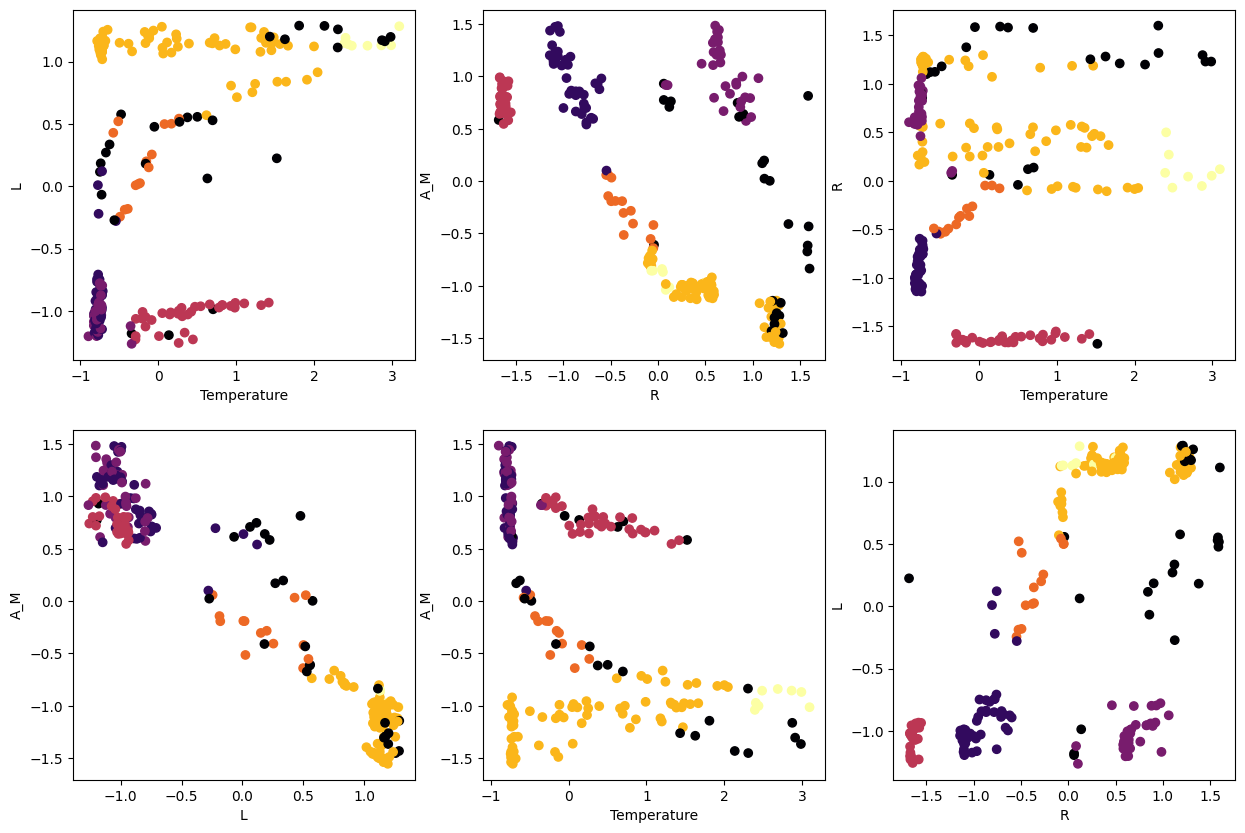
\includegraphics[width=1\linewidth]{figures/DBSCAN.png}
\end{figure}

Com esta configuração foram obtidos 27 \textit{outliers}\footnote{\texttt{str((categoriasDBSCAN == -1).sum())}} e 6 \textit{clusters}\footnote{\texttt{str(categoriasDBSCAN.max() + 1)}}, onde os \textit{outliers} são os pontos em preto nos gráficos. 
